\documentclass[ 
    aps,
    pra, 
    twocolumn,
    letterpaper,
    10pt,
    %draft,
    superscriptaddress, 
    showpacs,
    showkeys,
    notitlepage,
    amsmath, 
    amssymb, 
    floatfix 
]{revtex4-1} 
 
\usepackage{graphicx}% Include figure files
\usepackage{dcolumn}% Align table columns on decimal point
\usepackage{bm}% bold math
\usepackage{color}
\usepackage{amssymb}
\usepackage{dsfont}
\usepackage{amsmath}
\usepackage{hyperref}% add hypertext capabilities


\newcommand{\bel}{\begin{equation}}
\newcommand{\eel}{\end{equation}}
\newcommand{\be}{\begin{equation*}}
\newcommand{\ee}{\end{equation*}}
\newcommand{\bal}{\begin{eqnarray}}
\newcommand{\eal}{\end{eqnarray}}
\newcommand{\ba}{\begin{eqnarray*}}
\newcommand{\ea}{\end{eqnarray*}}

\newcommand{\no}{\noindent}

\newcommand{\refeq}[1]{Eq.~(\ref{#1})}
\newcommand{\reffig}[1]{Fig.~\ref{#1}}

\newcommand{\ev}[1]{\langle #1 \rangle}
\newcommand{\ket}[1]{| #1 \rangle}
\newcommand{\bra}[1]{\langle #1 |}
\newcommand{\Ev}[1]{\left\langle #1 \right\rangle}
\newcommand{\Ket}[1]{\left| #1 \right\rangle}
\newcommand{\Bra}[1]{\left\langle #1 \right|}
\newcommand{\+}{^\dagger}
\newcommand{\s}{^\ast}
\newcommand{\Tr}{\text{Tr}\,}

\newcommand{\br}{\mathbf{r}}
\newcommand{\bk}{\mathbf{k}}

\newcommand{\DD}{\mathcal{D}}
\newcommand{\PP}{\mathcal{P}}
\newcommand{\OO}{\mathcal{O}}
\newcommand{\eps}{\varepsilon}


\renewcommand{\d}[1]{\!d#1\,}

\newcommand{\pk}[1]{{\bf \color{blue} #1}}

 


\begin{document} 

%%%%%%%%%%%%%%%%%%%%%%%%%%%%%%%%%%%%%%%%
%%%%%%%%%%%%%%%%%%%%%%%%%%%%%%%%%%%%%%%%
\title{Supplementary Material for \\ 
Quantum network of atom clocks: a possible
implementation with neutral atoms }

\author{P. K\'{o}m\'{a}r}
\affiliation{Physics Department, Harvard University, Cambridge,
MA 02138, USA}

\author{T. Topcu}
\affiliation{Physics Department, Harvard University, Cambridge,
MA 02138, USA}
\affiliation{Department of Physics, University of Nevada, Reno, NV 89557, USA}
\affiliation{ITAMP, Harvard-Smithsonian Center for Astrophysics, Cambridge, MA 02138, USA}

\author{E. M. Kessler}
\affiliation{Physics Department, Harvard University, Cambridge,
MA 02138, USA}
\affiliation{ITAMP, Harvard-Smithsonian Center for Astrophysics, Cambridge, MA 02138, USA}

\author{A. Derevianko}
\affiliation{Physics Department, Harvard University, Cambridge,
MA 02138, USA}
\affiliation{Department of Physics, University of Nevada, Reno, NV 89557, USA}
\affiliation{ITAMP, Harvard-Smithsonian Center for Astrophysics, Cambridge, MA 02138, USA}

\author{V. Vuleti\'{c}}
\affiliation{Department of Physics and Research Laboratory of Electronics,
Massachusetts Institute of Technology, Cambridge, MA 02139, USA}

\author{J. Ye}
\affiliation{JILA, NIST, Department of Physics,  University of Colorado,
Boulder, CO 80309, USA}

\author{M. D. Lukin}
\affiliation{Physics Department, Harvard University, Cambridge,
MA 02138, USA}


\date{\today}


\maketitle

\section{Using the messenger atom}
With
proper optical control, we can entangle the ensembles by moving a single
Rydberg atom to the vicinity of each ensemble sequentially, such that its
blockade radius covers one of the clouds entirely.
Starting from the state
\bel
	\ket{g}^{
	nM}\big(\ket{s} + \ket{r_2}\big),
\eel
where the first $nM$ ket stand for the state of all atoms in the $M$
ensembles (each having $n$ atoms), and the last one represents the state of the
messenger atom. In a sequence, we imagine the messenger atom to be brought to
the vicinity of each ensemble, and the pulse sequence $[\pi/\sqrt{N}]_{g,r1},
[\pi]_{f,r1}$, creates an $f$ excitation, conditioned on the state of the
messenger atom. This plays out as follows
\bal
&&\rightarrow\ket{g}^{n(M-1)}\Big(\ket{1_f}_1\ket{s} + \ket{0}_1\ket{r_2}\Big)
\\
&&\rightarrow\ket{g}^{n(M-2)}\Big(\ket{1_f}_1\ket{1_f}_2\ket{s} +
\ket{0}_1\ket{0}_2\ket{r_2}\Big)
\\
&&\vdots
\\
&&\rightarrow \Big(\ket{1_f}^{M}\ket{s} + \ket{0}^M\ket{r_2}\Big),
\eal
which then only requires the messenger atom to be measured in the $\ket{\pm} =
(\ket{s} \pm \ket{r_2})$ basis, resulting in
\bel
	\rightarrow \ket{1_f}^{M} \pm \ket{0}^{M},
\eel
the required entangled state before the final GHZ extension step.

Disregarding the technical difficulties of trapping multiple atomic ensembles in
the same vacuum chamber, this entangling method has a higher fidelity than the
previous, photon-based, protocol, since it does not suffer from the errors
affecting the photon emission, propagation and detection. We model the
imperfections of this scheme by summing the error terms $\eps_1 + \eps_2 +
\eps_3$ only (from Eq.
(\ref{eq:f1}), (\ref{eq:f2}), (\ref{eq:f3})).

In section \ref{sec:Calculation for messenger atom}, we calculate a more
accurate result for the error contribution of imperfect blockade in the case of
placing the messenger atom close on the border of the cloud. We find  that this
increases the effect of the imperfect blockate by a factor of $\sim 2$,
resulting in an increase of $\sim 10\%$ in the total error.


\section{Overview of optimization}
In section \ref{sec:clock_precision}, we show that the figure of merit, the
precision gain with respect to non-entangled schemes, can be written as
\bel
\label{eq:G_first}
	G(N,E) = \frac{\pi}{8}e^{-E N}\sqrt{\frac{N}{\log N}},
\eel
where $N$ is the total number of entangled atoms in the global GHZ state, and
$E = E(n,\Omega)$ is the total error (contrast loss) divided by the total
number of atoms. $E$ depends on the number of atoms at a single clock, $n$, and the
Rabi-frequency of the dressing field used for local entanglement
growing.

We separate out the
minimization of $E$ (through finding the optimal $n, \Omega$
parameters), and the maximization of $G$ (through finding the optimal $N$). In
other words, we find
\bel
	G_\mathrm{max} = \max_N \,G\left(N,\,\min_{n,\Omega} E\right).
\eel
This two-step procedure gives identical results to the full optimization,
\bel
	G_\mathrm{max} = \max_{N,n,\Omega} G\Big(N, E(n,\Omega)\Big),
\eel
because both the maximum of $G$ and the optimal value of $N$ are
monotonically decreasing functions of $E$, for large $N$ (as can be seen from
\refeq{eq:G_first}).
We choose the two-step procedure because it is easier to carry out and
interpret.

 
\section{Local entangling errors }
The initial GHZ state is never perfect due to a series of imperfections in the
implementation. Here, we analyze the main errors responsible for lowering the
initial fidelity $F_\text{local} = [1+\exp(-\eps_\text{local})]/2$ of the GHZ
state of $n$ atoms, created via the conditional dressing scheme,  described in
the main article. We assume the following errors to be independent and small,
and we approximate $\eps_\text{local}$ with the sum
of the individual errors, $\sum_j \eps_j$. We evaluate the errors for a 2D
square lattice filled in a circular region and a 3D cubic lattice filled in a
spherical region (both of radius $R$). Where there is
a difference between the two cases, we give both results.


\subsection{Imperfect blockade}
\label{sec:imperfect_blockade}
If the blockade between the levels $r_1$ and $r_2$, $\Delta_{12}$, is not large
enough, the population transfer $g \rightarrow f$ happens even if $r_2$ is
populated by a single atom. Here, we analyze the effect of this imperfection.

Each pulse $\left[\frac{\pi}{\sqrt{n-j+1}}\right]_{g,r1}$, for $j=1,2,\dots n$
excites an average population of $\sim n
\left(\frac{\Omega}{2\Delta_{12}}\right)$ to the $r_1$ Rydberg state even if it
is detuned by $\Delta_{12}$ due to the interaction with the control atom being
in $r_2$ state. There are $n$ such pulses total, resulting in the error
\bel
	\eps_1 = \frac{n^2\Omega^2}{4} \Ev{\frac{1}{\Delta_{12}^2}},
\eel
where the average is taken over every pair of atoms in the ensemble. After
calculating this average for 2D and 3D spherical ensembles with uniform density,
we obtain
\bel
\label{eq:f1}
	\eps_1 = \left(\frac{\hbar a^3\Omega}{C_{12}^{(3)}}\right)^2\times 
	\left\{
	\begin{array}{ll}
		0.02818\, n^5 &\quad \text{(2D)} \\
		0.06079\, n^4 &\quad \text{(3D)}
	\end{array}
	\right.
	,
\eel
where $C_{12}^{(3)}$ is the dipole-dipole coefficient of the interaction between
$r_1$ and $r_2$, and $a$ is the lattice constant of the square (cubic) lattice
of the 2D (3D) ensemble.


\subsection{Decaying Rydberg states}
During the pulse sequence that induce the population transfer from $g$ to $f$,
the $r_1$ level is populated by an average of $1/2$ atoms. With constant
$\Omega$ Rabi frequency, the times of the pulse $j$ is $\frac{\pi}{\Omega
\sqrt{j}}$. The total accumulated error during the pulse sequence due to decay
or dephasing of $r_1$ Rydberg state is
\bel
	\eps_2^{(1)} = \frac{\gamma_1}{2} \frac{\pi}{\Omega}2\sum_{j=1}^n
	\frac{1}{\sqrt{j}} \approx \gamma \sqrt{n} \frac{2\pi}{\Omega}
\eel
where $\gamma_1$ is the total rate of loss (environment induced decay and
dephasing) from the Rydberg level $r_1$. The additional factor of 2 appears
because both the $g\rightarrow r_1$ and $r_1\rightarrow f$ transfers need to
happen.

In the meantime, the $r_2$ level is populated by a single atom. The decay and
dephasing of $r_2$, which we assume to be happening with rate $\gamma_2$ causes
error accumulation, which we approximate as
\bel
	\eps_2^{(2)} = \gamma_2 \frac{\pi}{\Omega}2\sum_{j=1}^n\frac{1}{\sqrt{j}}
	\approx \gamma \sqrt{n}\frac{4\pi}{\Omega}.
\eel

Although the two errors affect different components of the wavefunction, we use
their sum as an upper bound of their effect:
\bel
\label{eq:f2}
	\eps_2 = \eps_2^{(1)} + \eps_2^{(2)} = 6\pi \sqrt{n}\frac{\gamma}{\Omega}.
\eel

\subsection{Imperfect self-blockade}
During the excitation of the Rydberg state $r_1$, double excitations are mostly
shifted out of resonance by $\Delta_{11}$ due to the strong van der Waals
interaction between two $r_1$ atoms.
The time average of the population in the state where one Rydberg atom is excited is
$1/2$. The collective Rabi frequency between the 1-Rydberg state and the
2-Rydberg state is $\sqrt{2(n-1)}\Omega$. This translates to an average
population of $(n-1)\left(\frac{\Omega}{2\Delta_{11}}\right)$ during a single
pulse. Since there are $n$ such pulses during the population transfer from $g$
to $f$, the total accumulated error is
\bel
	\eps_3 \approx \frac{n^2\Omega^2}{4}\Ev{\frac{1}{\Delta_{11}^2}}.
\eel
After evaluating the average over all pair in the 2D (3D) ensemble, we
obtain
\bel
\label{eq:f3}
	\eps_3 = \left(\frac{\hbar a^6\Omega}{C_{11}^{(6)}}\right)^2 \times 
	\left\{
	\begin{array}{ll}
		0.01594\, n^8 &\quad \text{(2D)}\\
		0.05544\, n^6 &\quad \text{(3D)}\\
	\end{array}
	\right.
\eel
where $C_{11}^{(6)}$ is the van der Waals coefficient of the interaction between
two $r_1$ atoms, and $a$ is the lattice constant of the square (cubic)
lattice of the 2D (3D) ensemble.

\section{Non-local entangling errors}
Our protocol requires $K-1$ links to be set up between $K$ clocks. 
We denote the fidelity of a single connection by $F_\text{non-local} =
[1+\exp(-\eps_\text{non-local})]/2$,  and we approximate $\eps_\text{non-local}$
with the  sum of individual errors $\sum_i \eps_i$, detailed below.

\subsection{Imperfect blockade}
When exciting a single collective excitations, imperfect self-blockade can
result in leakage into double excited states. The probability of this can be
exponentially reduced by applying a smooth driving pulse. E.g., in case of a
Gaussian pulse of width $\tau$, and area $\pi$, exciting the $g
\rightarrow r_1$ transition is expected to be blocked when $r_2$ is populated, 
but it succeeds with probability $P_\text{double}$,
\bel
	P_\text{double} \approx \frac{\pi^2}{4}
	\exp\left[-\frac{(\Delta_{12}\tau)^2}{2}\right],
\eel
where $\Delta_{12} = C^{(3)}_{12}/(\hbar (2R)^3)$ is the minimal energy
shift in the ensemble due to the interaction of two atoms, one in $r_1$ and one
in $r_2$.
A detailed analysis of how different pulses affect the
transition probability can be found in \cite{Conover2011}. $P_\text{double} \ll
1$ requires
\bal
\label{eq:tau}
	&&\tau \leq \frac{\sqrt{2}}{\Delta_{12}} = 
	\left\{
	\begin{array}{ll}
	2 n^{3/2} \frac{\hbar a^3}{C^{(3)}_{12}} & \mathrm{(2D)} 
	\\
	2.7\, n  \frac{\hbar a^3}{C^{(3)}_{12}} & \mathrm{(3D)}
	\end{array}
	\right.
\eal 
in order to be small compared to the other errors.

\subsection{Rydberg state decay}
The $g\rightarrow r_1$ transition is driven with a pulse of duration $\tau$,
during which the $r_2$ level has a single excitation, which decays with rate
$\gamma_2$. The resulting error contribution, after all four photon pulses have
been generated, is
\bal
\label{eq:f4}
	&&\eps_4  = 4 \gamma_2 \tau = 
	\left\{
	\begin{array}{ll}
	8 n^{3/2} \frac{\hbar a^3 \gamma_2}{C_{12}^{(3)}} & \mathrm{(2D)}
	\\
	10.8\, n \frac{\hbar a^3 \gamma_2}{C_{12}^{(3)}} & \mathrm{(3D)}
	\end{array}
	\right.
\eal
where we used the expressions for $\tau$ from \refeq{eq:tau}.

\subsection{Photon propagation and detection errors}
The pairs of photons can get lost in the fiber during propagation and the
detection process (which is limited to 50\% for time-resolving detectors,  and
25\% for non-time-resolving ones). The two-photon heralding, however, detects
both of these errors. The remaining error comes from dark-counts of the
detectors. This affects a single link with the error
\bel
\label{eq:f5}
	\eps_5 \approx 4 \gamma_\text{dark}
	T_\text{detect} = \gamma_\text{dark} \frac{20}{n \gamma_e},
\eel
where $\gamma_\text{dark}$ is the dark count rate of the detectors,
 $T_\text{detect}$ (chosen such that a properly timed detector would have a
 chance to catch $1 -e^{-5} >  99\%$ of each photon) is the ``open time'' of the
 detector, and $\gamma_{e}$ is the spontaneous emission lifetime of the
 $\ket{e}\rightarrow \ket{g}$ transitions.
 The factor of $n$ is due to the collective enhancement of the said transition, and
 the factor of 4 is because four pulses are used in each connection.

We note that the probabilistic nature of the two-photon detection requires
repeating the connection steps between clocks every time it fails. With no
additional noise, this happens every second time, on average, requiring
resetting the $f$ and $s$ qubits in the two clocks in question. If the distance
between clocks is very large, photon propagation errors will increase the
average number of resets required for a single connection. Since every
qubit reset introduces additional errors, we want to minimize photon loss. If
the photon loss probabilit is $\eps$, the two-photon coincidence probabilit
becomes $\frac{1}{2}(1-\eps)^2$.

In the case of optical fibers (using an attenuation length of $L_\text{att} \sim
20$ km), we estimate $\eps \sim 1 - e^{-L/L_\text{att}}$, whose effect becomes
comparable to the ideal $50\%$ chance at around $L\sim 7\text{~km}$. Currently
we imagine our scheme working for terrestrial labs connected by fiber not longer
than this.

If clocks are operational on board of satellites, and optical links are
establised by actively stabilized telescopes, we estimate the photon loss
probability, due to diffraction, using the far-field (normalized) intensity
distribution (Airy-disk), $P(\theta) =
\frac{1}{\pi}\left(\frac{J_1(kR\sin\theta)}{\sin\theta}\right)^2$, where $J_1$
is a Bessel function. After approximating $\sin\theta\approx \theta$, we can
write the photon error probability as
\bel
	\eps = 1-2\intop_0^{kR^2/L}\d{x}\frac{(J_1(x))^2}{x},
\eel
where $R$ is the radius of the telescope objectives, and $k$ is the photon's
wavevector. Assuming $R\sim 1.25~\text{m}$ (Hubble's objective) and 3.11~eV
photon, the distance when photon loss error rate reaches $50\%$ is $1.5\times
10^7~\text{m} = 15,000~\text{km}$, which is larger that the average distance
between neighboring GPS satellites.

\subsection{Memory loss}
During the creation step of each link, the state $\ket{s}$ is used as memory.
On average, every link relies on one $s$ qubit. The time it takes to attempt the
creation of a link is $\sim 2L/c$, the time it takes for a light pulse to do a
round-trip between two stations.
During this time, quantum information is stored in qubit $s$, which is subject
decoherence happening at a rate $\gamma_s$.
The infidelity of the link originating from this error is
\bel
\label{eq:f6}
	\eps_6 = 4\frac{2L}{c}	\gamma_s.
\eel
State $\ket{f}$ is assumed to be a long-lived clock state, its decoherence rate
is negligible.

% In order to minimize the time each $s$ qubit is used to store quantum
% information, we assume that each site does the following. After attempting
% entanglement with the neighbors (using the $f$ qubit for the left neighbor, and
% the $s$ qubit for the right neighbor), four things can happen. If none of them
% or both of them succeeds the protocol  tries or performs a connection step right
% away. If only the left link succeeds then that is kept, and the right one
% (supported by the $s$ qubit) needs to be retried. If, however, the left one
% did not succeed but the right one does, then the site performs a swap between
% the $f$ and $s$ qubits, and further attempts to connect the left link will use
% the (no empty) $s$ qubit.

\subsection{Imperfect photon collection}
Collective enhancement makes the excited atom in state $\ket{e}$ decay
preferentially to $\ket{g}$, and emit a photon directly to the spatial mode
$\bk_e$, where $\bk_e$ is the spatial frequency of the collective mode $e$.
In the implementation with Yb atoms (discussed in Section
\ref{sec:Implementation}), the decay channel to $\ket{g}$ has a close
to unity branching ratio ($\zeta = 0.99$), but due to the finite size of the
ensemble, the photon collection efficiency is decreased.  The probability of not
capturing the emitted photon is
\bal
\label{eq:f7}
	\eps_7 \approx \frac{k_e^2 w^2}{3nI} =
	\left\{
	\begin{array}{ll}
		\frac{k_e^2a^2}{3\pi I}, & \text{(2D)}\\
		\frac{k_e^2a^2}{3 n^{1/3}I} \left(\frac{3}{4\pi}\right)^{2/3}, & \text{(3D)}
	\end{array}
	\right. 
\eal
where $w$ is the radius of the ensembles cross section perpendicular to $\bk_e$,
($w = a(n/\pi)^{1/2}$ for 2D, and $w = a(3n/(4\pi))^{1/3}$ for 3D.), and $k_e =
2\pi/ (1.4\,\mu\text{m})$, and $I\sim 100$ is the finesse of the cavity
that we envision using.

We note that in order to take full advantage of the collective enhancement
factor, $n$ in \refeq{eq:f7}, the phase matching condition has to be satisfied
between the two coherent fields, $g\rightarrow r_1$ (II) and $r_1\rightarrow e$
(III), and the spontaneously emitted photon $e\rightarrow g$ (IV). When an
optical cavity is placed around the ensemble, for the purpose of enhancing the
spontaneous emission, one need to carefully choose the wavevectors of field II
and III, such that $\bk_\text{IV} = \bk_\text{II} - \bk_\text{III}$, where
$\bk_\text{IV}$ is the wavevector of the emitted photon, which should be
paralell to the axis of the optical cavity, and the fields II and III should be
incident at a non-zero angle in order to not be blocked by the cavity. This is
possible only if the magnitude of $\bk_\text{III}$ is chosen to be slightly
larger than required to bridge the energy difference between $r_1$ and $e$.
Because the frequency of the state $e$ has a large spread (since it is very
short-lived), the rate of the $r_1\rightarrow e \rightarrow g$ transition will
not change significantly. (See \reffig{fig:cavity_fields}.)
 
\begin{figure}
\centering
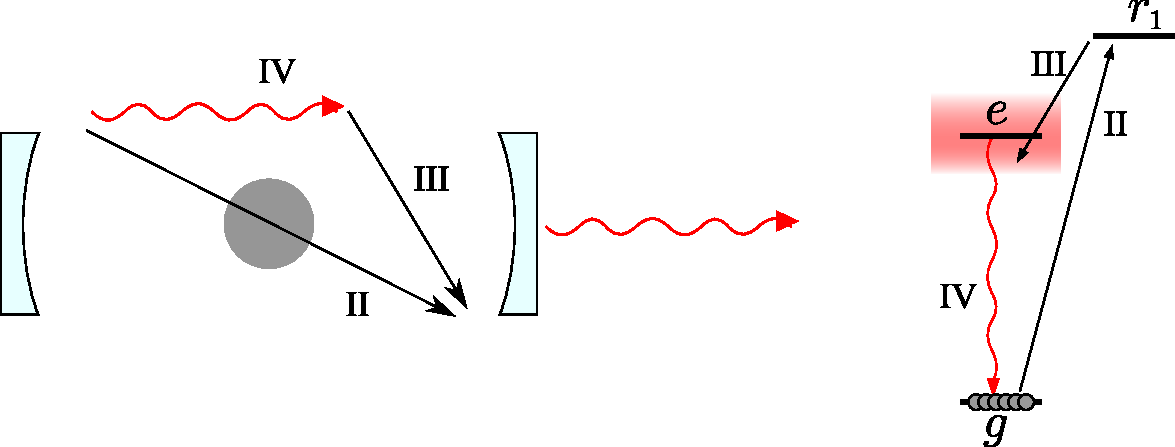
\includegraphics[width=0.40\textwidth]{./cavity_fields.pdf}
\caption[cavity_fields]{
\label{fig:cavity_fields}
The spontaneous emission can be enhanced by an optical
cavity only if the fields involved in the process are phase matched. This is
possible by setting the setting the frequence of field III slightly higher,
allowing the three fields to not be co-propagating. This way the coherent
fields can enter at an angle, and not be blocked by the high-finesse optical
cavity. The transition rate does not change considerably if the detuning of
III is smaller than the linewidth of level $e$.}
\end{figure}


% \subsection{Pulse area errors}
% Coherent pulses are required in each ensemble during the entangling procedure.
% We can express the fidelity of a single pulse as
% \bel
% 	|\ev{\psi_\text{target}|\psi}|^2 \sim 1-\delta^2/2,
% \eel
% where $\delta$ is the uncertainty of the pulse area. In order for this
% single-atom error to be smaller than $10^{-6}$, which means $\eps_9 =
% 10^{-6} n$, we need $\delta < 10^{-4}$.
% Although this can be challenging, with composite pulses it is feasible
% \cite{Chen2012}. 

\section{Implementation with Yb}
\label{sec:Implementation}
We imagine using the lower levels of neutral Yb for our protocol,  
$\ket{g} = \ket{6s^2({}^1\!S_0)}$, 
$\ket{f} = \ket{6s6p({}^3\!P_0)}$, 
$\ket{s} = \ket{6s6p({}^3\!P_2)}$ and 
$\ket{e} = \ket{6s6p({}^1\!P_1)}$, and 
two Rydberg levels 
$\ket{r_1} = \ket{6s\tilde n p_{m=+1}({}^1P_1)}$ and 
$\ket{r_2} = \ket{6s\tilde n s({}^3S_1)}$ 
with the same principle quantum number $\tilde n$. In the
case of the 2D lattice, we set the quantization axis perpendicular to the plane
in which the atoms reside, this way the dipole-dipole interaction between two
atoms, one in $\ket{r_2}$ and the other in $\ket{r_1}$, depends only on their
separation, $|\br_1 - \br_2|$. In the case of the 3D lattice, we rely on the
overwhelming strength of the Rydberg interaction to produce reliable blockade
even between atoms in different horizontal planes.

\subsection{Rydberg lifetimes}
We use the measured values from \cite{Fang2011} for principle quantum numbers
$\tilde n\sim 20-30$, and extrapolate the inverse lifetimes of the Rydberg
states
\bel
	\gamma_1\approx\gamma_2 = \gamma = \frac{8.403\times
	10^8~\text{s}^{-1}}{(\tilde n-4.279)^3}
\eel
where $\tilde n$ is the principle quantum number of the Rydberg orbit. Although
the measurement was carried out at $300~\text{K}$, the
contribution of the black body radiation (at $\tilde n \sim 20-30$) is
negligible even at this temperature, and therefore our extrapolation accurately
describes the effect of spontaneous emission on the lifetime. Cooling of the
radiation environment will be necessary to reach the above lifetime at $\tilde
n\sim 100$ and above. Furthermore, the photoionization rate from the $\tilde n
= 120$ Rydberg level, in a trapping field with $10^4~\text{W}/\text{cm}^2$
intensity, is five times smaller ($\gamma_\text{PI} \sim 110~\text{s}^{-1}$),
than the natural liftime ($\gamma \sim 540~\text{s}^{-1}$).


\subsection{Self-blockade, $\Delta_{11}$}
The long-range interaction between two $r_1$ atoms at a distance $R$ is
dominated by the van der Waals potential,
\bel
\label{eq:Delta_{11}(a)} 
	\Delta_{11}(R) = \frac{C_{11}^{(6)}}{\hbar R^6},
\eel
where $C_{11}^{(6)}$ strongly depends on the principle quantum number $\tilde
n$. We use results from \cite{Topcu2015}, and extrapolate the $C_{11}^{(6)}$
coefficient to high principle quantum numbers with the following formula,
\bel
	C_{11}^{(6)} = (-0.116 + 0.0339\, \tilde n) \,\tilde n^{11}\,
	\text{a.u.}
\eel
where the a.u. stands for atomic units, $E_h a_0^6 = 9.573\times
10^{-80}~\text{Jm}^6$, where $E_h$ is the Hartree energy and $a_0$ is the Bohr
radius.


\subsection{Cross-blockade, $\Delta_{12}$}
The long-range interaction between an $r_1$ and an $r_2$ atoms at a distance $R$
is dominated by the dipole-dipole interaction. We assume that the atoms are
confined in the $xy$ plane, and  because the $6s\tilde n p_{m=+1}$ state is
polarized in the $z$ direction, the interaction strength is independent of the
relative direction of one atom to the other.
\bel
\label{eq:Delta_{12}(a)}
	\Delta_{12}(R) = \frac{C_{12}^{(3)}}{\hbar R^3},
\eel
where $C_{12}^{(3)}$ depends strongly on the principle quantum number $\tilde
n$. We use results from \cite{Topcu2015}, and extrapolate the $C_{12}^{(3)}$
coefficient to high principle quantum numbers with the following formula,
\bel
	C_{12}^{(3)} = (0.149 + 0.00077\, \tilde n) \,\tilde n^{4}\,
	\text{a.u.}
\eel
where the a.u. stands for atomic units, $E_h a_0^3 = 6.460\times
10^{-49}~\text{Jm}^3$.

\subsection{Decay rates of lower levels}
The decay rate of $\ket{s} =\ket{6s6p\,,{}^3P_2}$ is $\gamma_s = 
[14.5\,\text{s}]^{-1} = 0.069\,\text{s}^{-1}$. The decay rate of the excited
state $\ket{e} = \ket{6s6p\,,{}^1P_1}$ is $\gamma_e  = 1.8\times
10^8\,\text{s}^{-1}$.


\subsection{Photon channels}
We assume that neighboring stations are $L < 10\,\text{km}$ apart from each
other, we neglect fiber and coupling loss. We further assume that single photon
detectors have a low dark count rate, i.e.
$\gamma_\text{dark}\approx 10\,\text{s}^{-1}$.


\section{Optimization}
The total initial imperfections of a GHZ state with $N$ atoms divided into $K$
clocks, each enclosing $M$ equal-sized ensembles (each of which contain $n$
atoms) is
\bal
	\eps_\text{tot} &=& (K-1)\eps_\text{non-local}
	+ MK \eps_\text{local} 
	\\ 
	&\approx & N\left(\frac{\eps_\text{local}}{n} +
	\frac{\eps_\text{non-local}}{Mn}\right) =: NE,
\eal
where the error contributions are $\eps_\text{local} = \eps_1 + \eps_2 +
\eps_3$, and $\eps_\text{non-local} = \eps_4 + \eps_5 + \eps_6 + \eps_7$, from
Eq.
(\ref{eq:f1}, \ref{eq:f2}, \ref{eq:f3}, \ref{eq:f4}, \ref{eq:f5}, \ref{eq:f6} and
\ref{eq:f7}).

It is clear that the larger $M$ is, the smaller the error is, however $nM$ (the
number of atoms in a single clock) is limited by the current state of technology
to $(nM)_\text{opt} \sim 2500$. Independently from the total atom number, $N$,
there is an optimal ensemble size, $n_\text{opt}$, for which $E$ (the total
error per atom) is minimal.
Below we find the optimal values of the parameters $\Omega$, (the
Rabi frequency the population transfer), and $n$ (the size of the each ensemble)
for fixed values of $\tilde n$ (the principle quantum number of the Rydberg
state) and  $a = 275.75\,\text{nm}$.

Using the following dimensionless variables, $\omega = \Omega / \gamma$,
$\delta_{11} = \frac{C_{11}^{(6)}}{\hbar a^6
\gamma}$ and $\delta_{12} = \frac{C_{12}^{(3)}}{\hbar a^3\gamma}$, we can write
the error per atom as $E: = \sum_i e_i$, where the terms
are $e_i = \eps_i/n$ for $i=1,2,3$ and $e_i = \eps_i/(Mn)_\text{opt} =
\eps_i/2500$ for $i=4,5,6,7$,
\bal
	e_1 &=& \left(\frac{\omega}{\delta_{12}}\right)^2\times 
	\left\{
	\begin{array}{ll}
		0.02818\, n^4 &\quad \text{(2D)} \\
		0.06079\, n^3 &\quad \text{(3D)}
	\end{array}
	\right.
	\\
	e_2 &=& \frac{6\pi}{n^{1/2}\omega}
	\\
	e_3 &=& \left(\frac{\omega}{\delta_{11}}\right)^2 \times 
	\left\{
	\begin{array}{ll}
		0.01594\, n^7 &\quad \text{(2D)}\\
		0.05544\, n^5 &\quad \text{(3D)}\\
	\end{array}
	\right.
	\\
	e_4 &=& \frac{1}{\delta_{12}\times 2500} \times
	\left\{
	\begin{array}{ll}
	8 \,n^{3/2} & \mathrm{(2D)}
	\\
	10.8 \,n & \mathrm{(3D)}
	\end{array}
	\right.
	\\
	e_5 &=&
	7.6\times 10^{-5}\, \frac{1}{2500\times n}
	\\
	e_6 &=& 1.8\times 10^{-5}/2500
	\\
	e_7 &=&
	\frac{1.532}{3\times 10^2 \times 2500} \times
	\left\{
	\begin{array}{ll}
		\frac{1}{\pi} & \text{(2D)}\\
		\frac{1}{n^{1/3}} \left(\frac{3}{4\pi}\right)^{2/3} &
		\text{(3D)}
	\end{array}
	\right.
\eal

\subsection{Optimal parameters}
We numerically minimized the sum, $E = \sum_i e_i$, by finding the optimal
values of $n$ for every $\tilde n \in [50,150]$, for $\omega = 10^5$.
(For $\tilde n = 120$, this Rabi frequency, $\Omega = 10^5\gamma =
2\pi\times 8.6~\text{MHz}$ is small enough, that the nearest
neighboring Rydberg level is well out of resonance: The level spacing is $\sim 2\pi\times
4~\text{GHz}$ between the $6s120s$ and $6s119s$ levels.)

The optimal number of atoms at a single ensemble
$n_\text{opt}$ are shown on \reffig{fig:opts}.
\begin{figure}[h] \centering
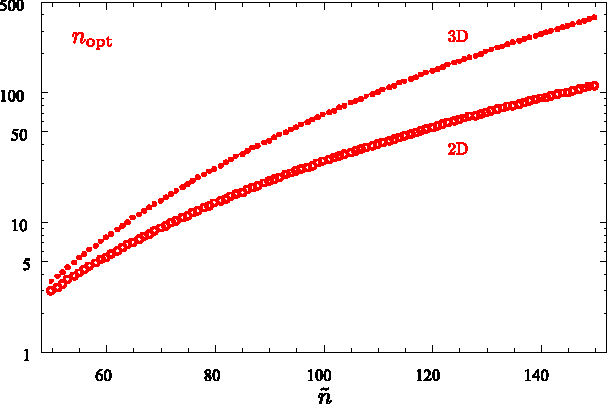
\includegraphics[width=0.48\textwidth]{./n_2d3d.pdf}  
\caption{
\label{fig:opts}
The
optimal number of atoms in a single ensemble $n$ is plotted as a function of the
principle quantum number of the Rydberg levels $\tilde n$, for the 2D and 3D
setup.}
\end{figure}

The
minimal error per atom $E_\text{min}$ is shown on
\reffig{fig:E_min}  as a function of $\tilde n$.
\begin{figure}[h]
\centering
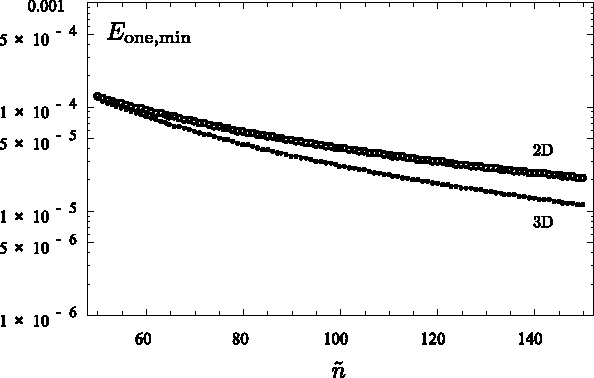
\includegraphics[width=0.48\textwidth]{./Eone_2d3d.pdf}
\caption{
\label{fig:E_min}
The minimized error contribution of a single atom as a function of the principle
quantum number of the Rydberg levels $\tilde n$, for the 2D and 3D setup.}
\end{figure}



\subsection{Comparison of error sources}
We compare the contributions of the different error terms $e_i$ to the total
error per atom, $\sum_i e_i$, for $\tilde n = 120$.
The different error terms contribute to the sum with amounts given in Table
\ref{table:errors_2D} and \ref{table:errors_3D}.
\begin{table}
\centering
\begin{tabular}{|l|c|c|}
\hline  
 Errors in 2D ensemble & error per atom & ratio in total\\
\hline
imperfect blockade ($e_1$) 	& $3.2 \times 10^{-6}$ 	& 11\%\\
Rydberg decay ($e_2$) 		& $2.5 \times 10^{-5}$ 	& 87\%\\
self-blockade ($e_3$) 		& $\sim 10^{-10}$ 	& $<0.1$\%\\
$r_2$ decay (non-local) ($e_4$) & $ \sim 10^{-11}$ 	& $<0.1$\%\\
photon detection ($e_5$) 	& $ \sim 10^{-12}$ 		& $<0.1$\%\\
memory error ($e_6$) 		& $ \sim 10^{-9}$ 	& $<0.1$\%\\
photon collection ($e_7$) & $6.5 \times 10^{-7}$ & $2$\%\\
\hline
total error per atom 		& $3.0 \times 10^{-5}$ & 100\%\\
\hline
\end{tabular}
\caption{
\label{table:errors_2D}
The absolute and relative contribution of the different error sources to the
total error per atom at $\tilde n = 120$, $\Omega = 
10^5\,\gamma$ and $n = n_\text{opt} = 54$.}
\end{table}

\begin{table}
\centering
\begin{tabular}{|l|c|c|}
\hline
 Errors in 3D ensemble & error per atom & ratio in total\\
\hline
imperfect blockade ($e_1$) 	& $2.6 \times 10^{-6}$ 	& 14\%\\
Rydberg decay ($e_2$) 		& $1.6 \times 10^{-5}$ 	& 86\%\\
self-blockade ($e_3$) 		& $\sim 10^{-11}$ 	& $<0.1$\%\\
$r_2$ decay (non-local) ($e_4$) & $ \sim 10^{-11}$ 	& $<0.1$\%\\
photon detection ($e_5$) 	& $ \sim 10^{-12}$ 		& $<0.1$\%\\
memory error ($e_6$) 		& $ \sim 10^{-8}$ 	& $<0.1$\%\\
photon collection ($e_7$) & $\sim 10^{-8}$ & $<0.1$\%\\
\hline
total error per atom 		& $1.8 \times 10^{-5}$ 	& 100\%\\
\hline
\end{tabular}
\caption{
\label{table:errors_3D}
The absolute and relative contribution of the different error sources to the
total error per atom at $\tilde n = 120$, $\Omega = 
10^5\,\gamma$ and $n = n_\text{opt} = 146$.}
\end{table}


\section{Clock precision}
\label{sec:clock_precision}

\subsection{Imperfect initialization}
The precision of an atomic clock employing a GHZ state of $N$ clock atoms is
limited by the initial imperfect creation of the GHZ state
described by the fidelity $F_N$ or contrast $c = 2F_N -1$.
We assume that an imperfect creation of the GHZ state result in the density
matrix 
\bel
	\rho_\text{non-pure} = c \ket{\Psi}
	\bra{\Psi}
	 + \frac{1-c}{2}\big(
	\ket{\mathbf{0}}\bra{\mathbf{0}} + \ket{\mathbf{1}}\bra{\mathbf{1}} \big),
\eel
where $\ket{\Psi} = \frac{\ket{\mathbf{0}} + \ket{\mathbf{1}}
}{\sqrt{2}}$, $\ket{\mathbf{0}} = \ket{0}^{\otimes N}$, $\ket{\mathbf{1}} =
\ket{1}^{\otimes N}$, and we assumed that only the relative phase between the
two components of the GHZ state changes to an unknown value,  but no
relaxation happens.

\subsection{Measurement}
After the interrogation time, the two components of the GHZ state pick up a
relative phase $N\phi$. $\ket{\Psi}\rightarrow \ket{\Psi_\phi} =
[\ket{\mathbf{0}} + e^{iN\phi}\ket{\mathbf{1}}]/\sqrt{2}$. Performing a perfect
single-atom $-\pi/2$ rotation around the $y$ axis for all atoms transforms this
into
\bel
	\ket{\Psi'_\phi} = \frac{1}{\sqrt{2^{N+1}}}\sum_{\{q_j\}} \left[1
	+(-1)^{\sum_j q_j} e^{iN\phi}\right] \ket{q_1,q_2, \dots q_N},
\eel
where $q_j\in\{0,1\}$ stands for the state of atom $j$. After this, we 
measure every atom (in the $z$-basis). The probability of any resulting
sequence, $\mathbf{q} = (q_1, q_2, \dots q_N) \in \{0,1\}^{\times N}$, is
\bel
	\PP(\mathbf{q} | \Psi'_\phi) = \frac{1}{2^{N+1}} \left[1 + (-1)^{\sum_j
	q_j} \cos(N\phi) \right],
\eel
and the probability of the parity, $p = \big(\sum_j q_j\big)\text{ mod } 2$, is
\bel
	\PP(p|\Psi'_\phi) = \frac{1 + (-1)^p\cos(N\phi)}{2}, \qquad p\in\{0,1\}.
\eel

On the other hand, these probabilities are different when they are conditioned
on being in the mixed part of the density matrix.
\bel
	\PP(\mathbf{q}|\rho_\text{mixed}) = \frac{1}{2^N}, \qquad
	\PP(p|\rho_\text{mixed}) = \frac{1}{2}
\eel
$\forall \mathbf{q}\in\{0,1\}^{\times N}$ and $\forall p\in\{0,1\}$, where
$\rho_\text{mixed} = [\ket{\mathbf{0}}\bra{\mathbf{0}} +
\ket{\mathbf{1}}\bra{\mathbf{1}}]/2$.

The resulting total probability is the weighted sum of the
two cases,
\bal
	\PP(p|\phi) &=& c\PP(p|\Psi'_\phi) + (1-c)\PP(p|\rho_\text{mixed})
	\quad \\
	&=&
	\frac{1 + c(-1)^p\cos(N\phi)}{2},
\eal
where $c = 2F_N -1$ is the
contrast of the interference fringes.


\subsection{Fisher information}
We rely on inferring the unknown phase $\phi$, from a series of parity
measurements, as described above. The information content  (about $\phi$) of a
single measured value $p$ is quantified by the Fisher information,
\bal
	\mathcal{F}(\phi) &=& \sum_{p\in\{0,1\}} \PP(p|\phi)
	\left[\ln\frac{d}{d\phi} \PP(p|\phi)\right]^2
	\\
	&=& N^2 \frac{\sin^2(N\phi)}{1/c^2 - \cos^2(N\phi)},
\eal
where the true value of the phase is $\phi$. The
average Fisher information is
\bel
	\overline{\mathcal{F}} = \frac{1}{2\pi}\intop_{-\pi}^{+\pi} \d{\phi}
	\mathcal{F}(\phi),
\eel
which we can evaluate in the limit of $c \ll 1$,
\bel
	\overline{\mathcal{F}} \approx \frac{1}{2\pi}\intop\d{\phi} c^2 \cos^2(N\phi) =
	\frac{N^2 c^2}{2}.
\eel
In the other limit, when $1 - c \ll 1$, $F(\phi)$ is approximately $c^2$
everywhere, except near the points where $\sin(N\phi)  = 0$. We approximate the
dip at $\phi = 0$ with
\bel
	\frac{\sin^2 x}{1/c^2 - \cos^2 x} \approx \frac{x^2}{\frac{1-c^2}{c^2} +
	x^2},\qquad \text{where }\; x = N\phi,
\eel
and the integral with
\bal
	\frac{\overline{\mathcal{F}}}{N^2} &\approx& c^2 -
	\frac{2}{2\pi}\int_{-\pi}^{+\pi}\d{x} \left(1- \frac{x^2}{\frac{1-c^2}{c^2} +
	x^2}\right)
	\\
	&=& c^2 -
	\frac{\sqrt{1-c^2}}{c}  \approx 1- \sqrt{2(1-c)},
\eal
where we have used that $F$ is periodic with period $2\pi/N$.

Using these two limits for the average Fisher information, we approximate it
with
\bal
\label{eq:overline_F}
	\overline{\mathcal{F}}
	&\approx&
	\left\{
	\begin{array}{ll}
		N^2 c^2/2 &,\quad \text{if}\quad c \leq 0.7, \\
		N^2\left(1 - \sqrt{2(1-c)}\right) &,\quad \text{if}\quad 1-c > 0.7.
	\end{array} 
	\right.
\eal
The quality of this approximation can be read off from \reffig{fig:Fisher_inf}
\begin{figure}[h]
\centering
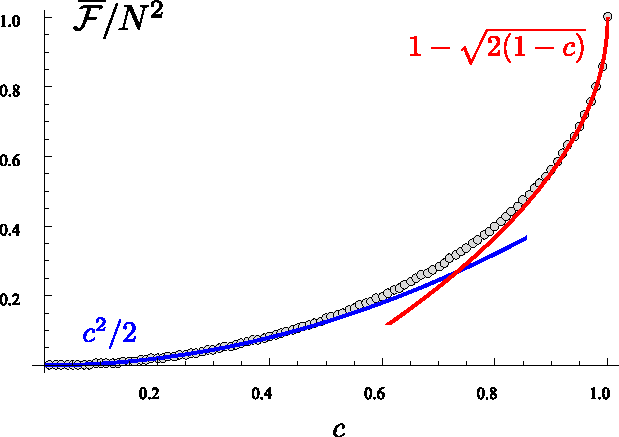
\includegraphics[width=0.4\textwidth]{./Fisher_inf.pdf}
\caption{
\label{fig:Fisher_inf}
Average Fisher information as a function of the contrast
$c$ (dots). It is well approximation by $c^2/2$ for $c < 0.6$ and by
$1-\sqrt{2(1-c)}$ for $c > 0.8$ (solid curves).} 
\end{figure}

\subsection{Cram\'{e}r-Rao bound}

The average Fisher information $\overline{\mathcal{F}}$ is a good measure of the
posterior uncertainty of the phase $\phi$, if the prior distribution of the
phase has been previously narrowed down to a small enough interval such that
its posterior is single peaked.
 In case of using the GHZ state, this requires a
very narrow prior to start with: $\phi \in [-\pi/N, +\pi/N]$. In our previous
work, we showed that this is possible by employing the atoms in a scheme using a
series of cascaded GHZ states \cite{Kessler2014}. The Cram\'{e}r-Rao bound on the
expected deviation of the estimated $\phi$ from the true one implies
\bel
	\Delta\phi = \sqrt{\Ev{(\phi_\text{estimate} - \phi_\text{true})^2} }\geq  
	\Big[\nu\overline{\mathcal{F}}\Big]^{-1/2},
\eel
where $\nu$ is the number of independent repetitions of the measurement. We are
going to assume equality to simplify our analysis.


\subsection{Allan deviation}
The average fractional frequency uncertainty of an atomic clock (with central
frequency $\omega_0$), averaged over a long time period $\tau$, is called
Allan deviation \cite{Kessler2014},
\bal
	\sigma = \frac{(\Delta\omega)_\tau}{\omega_0} \approx
	\frac{\Delta\phi_t/t}{\omega_0} \frac{1}{\sqrt{\tau/t}}
	\approx
	\frac{1}{\omega_0\sqrt{\tau}}\big[\nu t
	\overline{\mathcal{F}}\big]^{-1/2}\quad\quad
\eal
where $(\Delta \omega)_\tau =
\left|\frac{1}{\tau}\int\d{\tau'}\omega(\tau') - \omega_0\right|$ is the
deviation of the average frequency over time $\tau$, and $\Delta\phi_t$ is
the average deviation of the measured phase (from the true one) in a single
interrogation of length $t$. The $\sqrt{\tau/t}$ factor comes from the number of
independent repetitions of the same, $t$-long, interrogation cycle.

In Ref. \cite{Komar2014}, we showed that $\sigma$ can reach
\bel
	\sigma_\text{ent} \approx \frac{1}{\omega_0 \tau} \frac{8}{\pi}\frac{\sqrt{\log
	N}}{N},
\eel 
if $\tau < \gamma_\text{at}^{-1}/N$, the reduced atomic coherence time, and if
the contrast is perfect, ($c=1$). Using the approximation for
$\overline{\mathcal{F}}\approx N^2 c^2/2$,  and the fact that $\sigma \propto
[\overline{\mathcal{F}}]^{-1/2}\propto c^{-1}$, we can augment this result with
a $c$-dependence, and express the Allan deviation in the presence of
imperfections as
\bel
	\sigma_\text{ent}^\text{(imperfect)} = \sigma_\text{ent}/c = \frac{1}{c\omega_0
	\tau}\frac{8}{\pi}\frac{\sqrt{\log N}}{N}.
\eel


\subsection{Comparison to non-entangled interrogation}
Using the same number of atoms, $N$, we can arrange a measurement without using
any entanglement. This results in the Allan deviation of
\bel
\label{eq:sigma_single}
	\sigma_\text{non-ent}(\tau) \approx \frac{1}{\omega_0 \tau\sqrt{N}},\qquad
	\text{if}\quad \tau < 1/\gamma_\text{LO},
\eel
where $\gamma_\text{LO}^{-1}$ is the laser coherence time.
This, representing the standard quantum limit (SQL), is expected to be larger
than the Allan deviation corresponding to the GHZ state scheme, which is almost
at the Heisenberg limit. The precision gain of the GHZ scheme over the
non-entangled one is
\bel
\label{eq:gain_supp}
	G = \frac{\sigma_\text{non-ent}}{\sigma_\text{ent}/c} =
	(2F_N -1)\frac{\pi}{8}\sqrt{\frac{N}{\log{N}}}.
\eel
Since the fidelity $F_N$ decreases with increasing $N$, there exist an optimal
$N_\text{opt}$, for which the gain $G$ is maximal.

\subsection{Optimal clock network size}
If each clock runs with the optimal setup ($n_\text{opt}$),
then the total error per atom, $E$, is minimal, and the total fidelity can be
written as $F_N = \left[1+e^{-E_\text{min}N}\right]/2$. Plugging this into
\refeq{eq:gain_supp} gives
\bel
	G = e^{-E_\text{min} N} \frac{\pi}{8}\sqrt{\frac{N}{\log N}},
\eel 
which takes its maximum at $N = N_\text{max} \approx \frac{1}{2E_\text{min}}$,
giving $G_\text{max} \approx \frac{\pi}{8}
\left[E_\text{min}\log\left(\frac{1}{2E_\text{min}}\right)\right]^{-1/2}$.
In the meantime the number of atoms at a single clock is  $\sim 2500$.
As a result the optimal number of clocks becomes 
\bel
	K_\text{opt} \sim \frac{N_\text{max}}{2500}.
\eel

On \reffig{fig:K}, we plot $N_{\text{max}}$, $n_\text{opt}$, and
$K_\text{opt}$ as a function of the principle quantum number of the
Rydberg states $\tilde n$.
\begin{figure}[h]
\centering
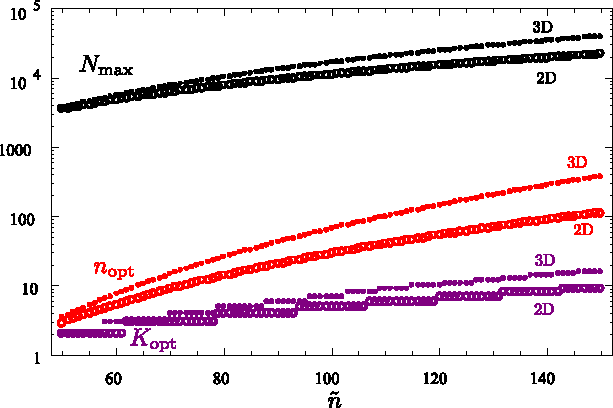
\includegraphics[width=0.48\textwidth]{./NnK_2d3d.pdf}
\caption{
\label{fig:K}
The optimal total number of entangled atoms in the network $N_\text{max}$ and
the number of atoms at a single clock $n_\text{opt}$ as a function of the
principle quantum number $\tilde n$. The thin dotted lines show the multiples of
$n_\text{opt}$. The optimal number of clocks, $K_\text{opt} \sim
N_\text{max}/2500$ is written on the corresponding regions of $\tilde n$, for
the 2D and 3D setup.}
\end{figure}
For $\tilde n = 120$, we find $N_\text{max} \approx 15000$ (2D) and $\approx
25000$ (3D). Using the $n_\text{opt}$ values from before ($\approx 50$ and
$\approx 150$), we find $K_\text{opt} \sim 6$ and $\sim 10$, for 2D and 3D,
respectively. 

With the optimal architecture, we can plot the maximal gain $G_\text{max}$
(compared to the non-entangled scheme using the same number of atoms) as a
function of principle quantum number $\tilde n$. 
This is shown on \reffig{fig:gain}.
\begin{figure}[h] 
\centering
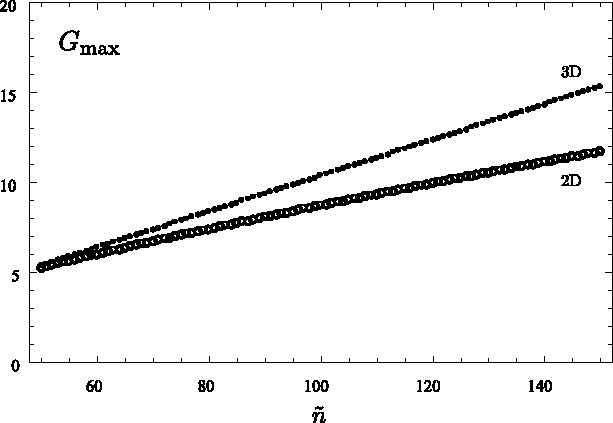
\includegraphics[width=0.48\textwidth]{./gain_2d3d.pdf}
\caption{
\label{fig:gain}
Maximal gain over the non-entangled scheme provided by the optimal entangled
clock network architecture as a function of principle quantum number of the
Rydberg states $\tilde n$, for the 2D and 3D setup.}
\end{figure}
For $\tilde n = 120$, the gain is $G_\text{max} = 10$ (2D) and $12$ (3D).


\section{GHZ generation timescale}
The global GHZ state needs to be set up at the beginning of every clock cycle.
The average total time required to perform every step successfully is determined
by the time it takes the longest step (photon propagation), and how many times
this has to be repeated, after heralding indicates (partial) failure.

Ideally photon propagation and classical communication takes $2L/c$ time, where
$L$ is the distance between neighboring clocks and $c$ is the speed of light
(in the fiber). For clocks separated by $5~\text{km}$, this is
$0.17~\mu\text{s}$.

However, the two-photon detection process is probabilistic, which (for
distances $\sim 5$~km) succeeds only every fourth time $p=1/4$. This means that
the probability that a single link still fails to establish after the $t$th
trial is $(1-p)^t$. Conversely, the probability that it succeeds some time
before or on the $t$th trials is $1-(1-p)^t$. The probability that all $K-1$
links succeed is $\left[1-(1-p)^t\right]^{K-1}$, and the probability that at
least one of them still didn't succeed in $t$ trails is $1 -
\left[1-(1-p)^t\right]^{K-1}$. Now, this is exactly the probability that we need
to try more than $t$ times before globally succeeding. This means we can write
the probability of globally succeeding exactly on the $t$the trial is:
\bal
	\PP(t) &=& \PP(\text{no success in $t-1$ trial}) \nonumber\\
	&& - \PP(\text{no
	success in $t$ trials}) = \nonumber\\
	&=& \left\{1 - \left[1-(1-p)^{t-1}\right]^{K-1}\right\} \nonumber\\
	&& - \left\{1 - \left[1-(1-p)^t\right]^{K-1}\right\}
\eal
The expectation value of $t$ (number of required repetitions) can be calculated
numerically for $p=0.25$ and $K=10$ is $\ev{t} = 10.33$.

Multiplying the ideal wait time with this expected number of repetitions gives
$1.75\mu\text{s}$ average time required to set up the global GHZ state.


\section{Prospects with current experimental technology}  
In our analysis above, we investigated the effects of noise sources which are
fundamental to photons and Rydberg states. This result, however, posits only 
a lower bound to infidelity. Realizing our scheme with current
experimental technology is more challenging than it may seem, due to additional
imperfections of the implementation. 

Out of the five steps of our protocol, generating the spin-photon
entangled states (step 2) and producing the entangled states between neighboring
but remote atomic ensembles (step 3) are the most restrictive. Although
possible, the overall efficiency is low ($\sim 70\%$ for
non-local entangling \cite{Vittorini2014}, and $\sim 90\%$ for Rydberg
efficiency \cite{Labuhn2014}).
This greatly limits the possibility of demonstrating overall precision boost
with current experimental technology.


\section{Calculating $\ev{1/\Delta_{12}^2}$}
\label{sec:calc_Delta12}
Here, we calculate the average of 
\bel
	\frac{1}{\Delta_{12}^2} = \left(\frac{\hbar}{C_{12}^{(3)}}\right)^2 |\br_1 -
	\br_2|^6
\eel
for all $(j,k)$ pairs in
an ensemble of $n$ atoms, trapped in a (square or cubic)lattice with
periodicity $a$, uniformly filling a circular 2D (spherical 3D) region of radius
$R$.

Averaging over the cloud of atoms, can be approximated by the following integral
\bel
\label{eq:SI_Delta12}
	\Ev{\frac{1}{\Delta_{12}^2}} \approx \left(\frac{\hbar}{C_{12}^{(3)}}\right)^2
	\underbrace{\frac{1}{V^2}\intop_V\d{^\eta \br_j}\intop_V\d{^\eta \br_k}|\br_j -
	\br_j|^6}_{R^6 I}
\eel
where $\eta = 2,3$,  $V$ is the filled region, of radius $R$, in a (2D or 3D)
lattice.

We introduce new variables $x = |\br_j - \br_k|$, $r = |\br_j|$, and use
the circular symmetry of the cloud and the spherical symmetry of the
interaction, to turn the integrals into one dimensional ones.
\bal
	R^6 I_\text{2D} &=& \frac{1}{(\pi R^2)^2}\intop_0^R\d{r}2\pi r
	\intop_{0}^{2R}\d{x} S_R(r,x) x^6,
	\\
	R^6 I_\text{3D} &=& \frac{1}{(4\pi R^3/3)^2}\intop_0^R\d{r}4\pi r^2
	\intop_{0}^{2R}\d{x} A_R(r,x) x^6,
\eal
where the
weighting factor $S_R(r,x)$ is the length of the segment of a circle of radius
$x$, centered at $r$ distance from the origin that lies inside the 2D cloud of
radius $R$. (See \reffig{fig:circles}).
It can be written as
\bal
\label{eq:S_R}
	S_R(r,x) &=&
	\left\{
	\begin{array}{ll}
		2\pi x &,\, \text{if}\; x < R-r \\ 
		0 &,\, \text{if}\; R+r < x \\
		2x \arccos\left(\frac{x^2 + r^2 - R^2}{2xr}\right) &,\, \text{otherwise}
	\end{array}
	\right.\quad
\eal
\begin{figure}[h]
\centering
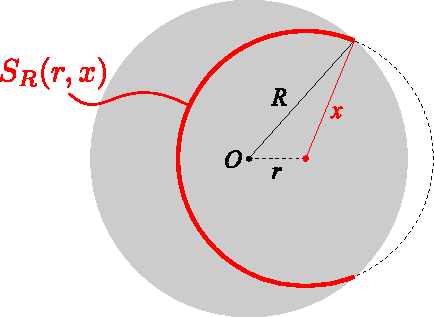
\includegraphics[width=0.30\textwidth]{./circles.pdf}
\caption{
\label{fig:circles}
The length of the circle segment of radius $x$ lying inside the cloud of radius
$R$, $S_R(r,x)$, is between 0 and $2\pi x$ for $R-r < x < R+r$, where $r$ is
the separation between the centers.}
\end{figure}
Similarly, $A_R(r,x)$ is the area of a spherical surface or radius
$x$ centered  $r$ distance from the center of the 3D
cloud located inside the cloud.
It can be written as
\bal
\label{eq:A_R}
	A_R(r,x) &=&
	\left\{
	\begin{array}{ll}
		4\pi x^2 &,\, \mathrm{if}\; x < R-r \\
		0 &, \, \mathrm{if}\; R+r < x\\
		\pi\frac{x}{r}\left[R^2 - (x-r)^2\right] &,\, \mathrm{otherwise}
	\end{array}
	\right.\quad
\eal
Using the explicit expressions of \refeq{eq:S_R} and (\ref{eq:A_R}), we can
write
\bal
	I_\text{2D} &=& 4\intop_0^1\d{\rho}\rho \intop_0^{1-\rho}\d{\xi} \xi^7 + \\
	&&
	+ 4 \intop_0^1 \d{\rho}\rho \intop_{1-\rho}^{1+\rho}\d{\xi} \frac{1}{\pi}\xi^7
	\arccos\left(\frac{\xi^2+\rho^2 -1}{2\rho\xi}\right),
	\\
	I_\text{3D} &=& 9\intop_0^1\d{\rho}\rho^2\intop_{0}^{1-\rho}\d{\xi} \xi^8 + \\
	&&
	+ 9 \intop_0^1\d{\rho}\rho^2\intop_{1-\rho}^{1+\rho}\d{\xi}
	\frac{1}{4}\frac{\xi^7}{\rho}\left[1 - \left(\xi-\rho\right)^2\right],
\eal
which we numerically evaluate and find $I_\text{2D} = 3.5$, and
$I_\text{3D} = 4.27$.

Using that $\pi R^2 = n a^2$ (in 2D) and $4\pi R^3/3 = n a^3$ (in 3D), we can
obtain the expressions in \refeq{eq:f1}.

\section{Calculating $\ev{1/\Delta_{12}^2}$ for messenger atom}
\label{sec:Calculation for messenger atom}
When a messenger atom is used, we imaging placing it just outside the
amotic cloud. This changes the expression from \refeq{eq:SI_Delta12} to
\bel
	\Ev{\frac{1}{\Delta_{12}^2}} \approx \left(\frac{\hbar}{C_{12}^{(3)}}\right)^2
	\frac{1}{V} \intop_V\d{^\eta \br} |\br - \br_m|^6,
\eel
where $\br$ is the position of an atom in the cloud, and $\br_m$ is the
messenger atom's position. Following the same steps as in the previous section,
we need to calculate the following integrals:
\bal
	R^6 J_\text{2D} &=& \frac{1}{\pi R^2} \intop_0^{2R}\d{x} S_R(r_m,x) x^6,
	\\
	R^6 J_\text{3D} &=& \frac{1}{4\pi R^3/3} \intop_0^{2R} \d{x}A_{R}(r_m, x) x^6.
\eal
Using that $r_m = |\br_m| = R$, and the expressions for $S_R$ and $A_R$, we get
$J_\text{2D} = 8.75$ and $J_\text{3D} = 4.27$.

This results in a $\sim~2$-fold increase of the imperfect blockade error,
raising its contribution to 20-30\% in the total error, and increasing it by $\sim 10\%$

\section{Calculating $\ev{1/\Delta_{11}^2}$}
Following the same line of thoughts as in the previous section, we can write the
average as
\bel
	\Ev{\frac{1}{\Delta_{11}^2}} = \approx
	\left(\frac{\hbar}{C_{11}^{(6)}}\right)^2
	\underbrace{\frac{1}{V^2}\intop_V\d{^\eta \br_j}\intop_V\d{^\eta \br_k}|\br_j
	- \br_j|^{12}}_{R^{12} J}
	\frac{1}{V^2}. 
\eel
The integral $J$ can be evaluated following the same methods as in the previous
section, and we obtain $J_\text{2D} = 61.29$, $J_\text{3D} = 68.26$.

Using that $\pi R^2 = n a^2$ (in 2D) and $4\pi R^3/3 = n a^3$ (in 3D), we can
obtain the expressions in \refeq{eq:f3}.



% \bibliography{Rydberg_GHZ}

%merlin.mbs apsrev4-1.bst 2010-07-25 4.21a (PWD, AO, DPC) hacked
%Control: key (0)
%Control: author (8) initials jnrlst
%Control: editor formatted (1) identically to author
%Control: production of article title (-1) disabled
%Control: page (0) single
%Control: year (1) truncated
%Control: production of eprint (0) enabled
\begin{thebibliography}{7}%
\makeatletter
\providecommand \@ifxundefined [1]{%
 \@ifx{#1\undefined}
}%
\providecommand \@ifnum [1]{%
 \ifnum #1\expandafter \@firstoftwo
 \else \expandafter \@secondoftwo
 \fi
}%
\providecommand \@ifx [1]{%
 \ifx #1\expandafter \@firstoftwo
 \else \expandafter \@secondoftwo
 \fi
}%
\providecommand \natexlab [1]{#1}%
\providecommand \enquote  [1]{``#1''}%
\providecommand \bibnamefont  [1]{#1}%
\providecommand \bibfnamefont [1]{#1}%
\providecommand \citenamefont [1]{#1}%
\providecommand \href@noop [0]{\@secondoftwo}%
\providecommand \href [0]{\begingroup \@sanitize@url \@href}%
\providecommand \@href[1]{\@@startlink{#1}\@@href}%
\providecommand \@@href[1]{\endgroup#1\@@endlink}%
\providecommand \@sanitize@url [0]{\catcode `\\12\catcode `\$12\catcode
  `\&12\catcode `\#12\catcode `\^12\catcode `\_12\catcode `\%12\relax}%
\providecommand \@@startlink[1]{}%
\providecommand \@@endlink[0]{}%
\providecommand \url  [0]{\begingroup\@sanitize@url \@url }%
\providecommand \@url [1]{\endgroup\@href {#1}{\urlprefix }}%
\providecommand \urlprefix  [0]{URL }%
\providecommand \Eprint [0]{\href }%
\providecommand \doibase [0]{http://dx.doi.org/}%
\providecommand \selectlanguage [0]{\@gobble}%
\providecommand \bibinfo  [0]{\@secondoftwo}%
\providecommand \bibfield  [0]{\@secondoftwo}%
\providecommand \translation [1]{[#1]}%
\providecommand \BibitemOpen [0]{}%
\providecommand \bibitemStop [0]{}%
\providecommand \bibitemNoStop [0]{.\EOS\space}%
\providecommand \EOS [0]{\spacefactor3000\relax}%
\providecommand \BibitemShut  [1]{\csname bibitem#1\endcsname}%
\let\auto@bib@innerbib\@empty
%</preamble>
\bibitem [{\citenamefont {Conover}(2011)}]{Conover2011}%
  \BibitemOpen
  \bibfield  {author} {\bibinfo {author} {\bibfnamefont {C.~W.~S.}\
  \bibnamefont {Conover}},\ }\href {\doibase 10.1103/PhysRevA.84.063416}
  {\bibfield  {journal} {\bibinfo  {journal} {Phys. Rev. A}\ }\textbf {\bibinfo
  {volume} {84}},\ \bibinfo {pages} {1} (\bibinfo {year} {2011})}\BibitemShut
  {NoStop}%
\bibitem [{\citenamefont {Fang}\ \emph {et~al.}(2001)\citenamefont {Fang},
  \citenamefont {Xie}, \citenamefont {Zhang}, \citenamefont {Hu},\ and\
  \citenamefont {Liu}}]{Fang2011}%
  \BibitemOpen
  \bibfield  {author} {\bibinfo {author} {\bibfnamefont {D.-W.}\ \bibnamefont
  {Fang}}, \bibinfo {author} {\bibfnamefont {W.-J.}\ \bibnamefont {Xie}},
  \bibinfo {author} {\bibfnamefont {Y.}~\bibnamefont {Zhang}}, \bibinfo
  {author} {\bibfnamefont {X.}~\bibnamefont {Hu}}, \ and\ \bibinfo {author}
  {\bibfnamefont {Y.-Y.}\ \bibnamefont {Liu}},\ }\href {\doibase
  10.1016/S0022-4073(00)00096-0} {\bibfield  {journal} {\bibinfo  {journal}
  {Journal of Quantitative Spectroscopy and Radiative Transfer}\ }\textbf
  {\bibinfo {volume} {69}},\ \bibinfo {pages} {469�473} (\bibinfo {year}
  {2001})}\BibitemShut {NoStop}%
\bibitem [{\citenamefont {Turker~Topcu}(2015)}]{Topcu2015}%
  \BibitemOpen
  \bibfield  {author} {\bibinfo {author} {\bibfnamefont {A.~D.}\ \bibnamefont
  {Turker~Topcu}},\ }\href {http://arxiv.org/abs/1505.07152} {\bibfield
  {journal} {\bibinfo  {journal} {arXiv:1505.07152}\ } (\bibinfo {year}
  {2015})}\BibitemShut {NoStop}%
\bibitem [{\citenamefont {Kessler}\ \emph {et~al.}(2014)\citenamefont
  {Kessler}, \citenamefont {K\'{o}m\'{a}r}, \citenamefont {Bishof},
  \citenamefont {Jiang}, \citenamefont {S{\o}rensen}, \citenamefont {Ye},\ and\
  \citenamefont {Lukin}}]{Kessler2014}%
  \BibitemOpen
  \bibfield  {author} {\bibinfo {author} {\bibfnamefont {E.~M.}\ \bibnamefont
  {Kessler}}, \bibinfo {author} {\bibfnamefont {P.}~\bibnamefont
  {K\'{o}m\'{a}r}}, \bibinfo {author} {\bibfnamefont {M.}~\bibnamefont
  {Bishof}}, \bibinfo {author} {\bibfnamefont {L.}~\bibnamefont {Jiang}},
  \bibinfo {author} {\bibfnamefont {A.~S.}\ \bibnamefont {S{\o}rensen}},
  \bibinfo {author} {\bibfnamefont {J.}~\bibnamefont {Ye}}, \ and\ \bibinfo
  {author} {\bibfnamefont {M.~D.}\ \bibnamefont {Lukin}},\ }\href {\doibase
  10.1103/PhysRevLett.112.190403} {\bibfield  {journal} {\bibinfo  {journal}
  {Phys. Rev. Lett.}\ }\textbf {\bibinfo {volume} {112}},\ \bibinfo {pages}
  {190403} (\bibinfo {year} {2014})}\BibitemShut {NoStop}%
\bibitem [{\citenamefont {K\'{o}m\'{a}r}\ \emph {et~al.}(2014)\citenamefont
  {K\'{o}m\'{a}r}, \citenamefont {Kessler}, \citenamefont {Bishof},
  \citenamefont {Jiang}, \citenamefont {S{\o}rensen}, \citenamefont {Ye},\ and\
  \citenamefont {Lukin}}]{Komar2014}%
  \BibitemOpen
  \bibfield  {author} {\bibinfo {author} {\bibfnamefont {P.}~\bibnamefont
  {K\'{o}m\'{a}r}}, \bibinfo {author} {\bibfnamefont {E.~M.}\ \bibnamefont
  {Kessler}}, \bibinfo {author} {\bibfnamefont {M.}~\bibnamefont {Bishof}},
  \bibinfo {author} {\bibfnamefont {L.}~\bibnamefont {Jiang}}, \bibinfo
  {author} {\bibfnamefont {A.~S.}\ \bibnamefont {S{\o}rensen}}, \bibinfo
  {author} {\bibfnamefont {J.}~\bibnamefont {Ye}}, \ and\ \bibinfo {author}
  {\bibfnamefont {M.~D.}\ \bibnamefont {Lukin}},\ }\href {\doibase
  10.1038/nphys3000} {\bibfield  {journal} {\bibinfo  {journal} {Nature
  Physics}\ }\textbf {\bibinfo {volume} {10}},\ \bibinfo {pages} {582}
  (\bibinfo {year} {2014})}\BibitemShut {NoStop}%
\bibitem [{\citenamefont {Vittorini}\ \emph {et~al.}(2014)\citenamefont
  {Vittorini}, \citenamefont {Hucul}, \citenamefont {Inlek}, \citenamefont
  {Crocker},\ and\ \citenamefont {Monroe}}]{Vittorini2014}%
  \BibitemOpen
  \bibfield  {author} {\bibinfo {author} {\bibfnamefont {G.}~\bibnamefont
  {Vittorini}}, \bibinfo {author} {\bibfnamefont {D.}~\bibnamefont {Hucul}},
  \bibinfo {author} {\bibfnamefont {I.~V.}\ \bibnamefont {Inlek}}, \bibinfo
  {author} {\bibfnamefont {C.}~\bibnamefont {Crocker}}, \ and\ \bibinfo
  {author} {\bibfnamefont {C.}~\bibnamefont {Monroe}},\ }\href {\doibase
  10.1103/PhysRevA.90.040302} {\bibfield  {journal} {\bibinfo  {journal} {Phys.
  Rev. A}\ }\textbf {\bibinfo {volume} {90}},\ \bibinfo {pages} {040302}
  (\bibinfo {year} {2014})}\BibitemShut {NoStop}%
\bibitem [{\citenamefont {Labuhn}\ \emph {et~al.}(2014)\citenamefont {Labuhn},
  \citenamefont {Ravets}, \citenamefont {Barredo}, \citenamefont {B\'eguin},
  \citenamefont {Nogrette}, \citenamefont {Lahaye},\ and\ \citenamefont
  {Browaeys}}]{Labuhn2014}%
  \BibitemOpen
  \bibfield  {author} {\bibinfo {author} {\bibfnamefont {H.}~\bibnamefont
  {Labuhn}}, \bibinfo {author} {\bibfnamefont {S.}~\bibnamefont {Ravets}},
  \bibinfo {author} {\bibfnamefont {D.}~\bibnamefont {Barredo}}, \bibinfo
  {author} {\bibfnamefont {L.}~\bibnamefont {B\'eguin}}, \bibinfo {author}
  {\bibfnamefont {F.}~\bibnamefont {Nogrette}}, \bibinfo {author}
  {\bibfnamefont {T.}~\bibnamefont {Lahaye}}, \ and\ \bibinfo {author}
  {\bibfnamefont {A.}~\bibnamefont {Browaeys}},\ }\href {\doibase
  10.1103/PhysRevA.90.023415} {\bibfield  {journal} {\bibinfo  {journal} {Phys.
  Rev. A}\ }\textbf {\bibinfo {volume} {90}},\ \bibinfo {pages} {023415}
  (\bibinfo {year} {2014})}\BibitemShut {NoStop}%
\end{thebibliography}% 


\end{document}
